\documentclass[UTF8]{ctexart}
\usepackage{graphicx}
\usepackage{amsmath}
\usepackage{bibentry,natbib}
\usepackage{fancyhdr}

\title{C++ Reference}
\author{BrightHush}
\date{\today}

\begin{document}
\maketitle
\tableofcontents

\pagestyle{fancy}
\cfoot{\thepage}

\newcommand{\figref}[1]{\figurename~\ref{#1}}
%\begin{figure}[h!]
%    \centering     
%    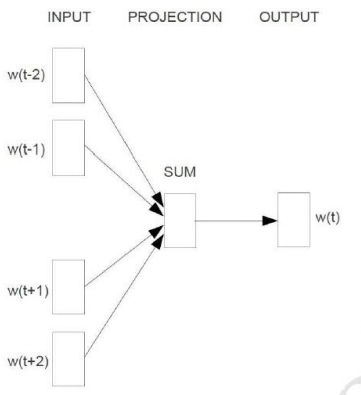
\includegraphics[width=0.5\textwidth]{cbow}   
%    \caption{\label{Fig:CBOW}CBOW Architecture} 
%\end{figure}

\section{class std::string}
\verb{<string> \\
typedef basic_string<char> string;
}

\section{References}
\begin{itemize}
\item[1] word2vec 中的数学原理详解, \\
\url{http://blog.csdn.net/itplus/article/details/37969519}.
\end{itemize}

\end{document}
